\documentclass[tikz]{standalone}

\usepackage{amsfonts}
\usetikzlibrary{decorations.pathreplacing}
\usetikzlibrary{hobby}

\begin{document}
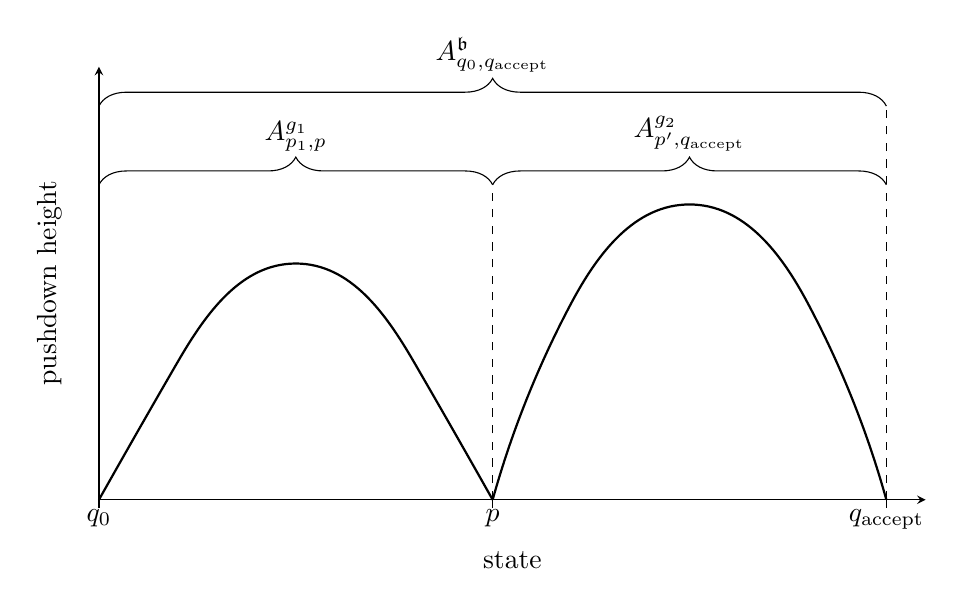
\begin{tikzpicture}[>=stealth]

\draw [<->]
	(0,5.5) to node [rotate=90,above=1em]  {pushdown height}
	(0,0)  to node [below=1.5em] {state}
	(10.5,0);

\draw (0,0) node [below] {$q_0$};

\draw (5,0) node [below] {$p$};

\draw (10,0) node [below] {$q_\mathrm{accept}$};

\draw (0,0) to +(0,-0.1);
\draw (5,0) to +(0,-0.1);
\draw (10,0) to +(0,-0.1);

\draw [thick] (0,0) to [curve through={
	   (1,  1.75)
	.. (2.5,3)
	.. (4,  1.75)
}] (5,0);
\draw [thick] (5,0) to [curve through={
	   (6,  2.5)
	.. (7.5,3.75)
	.. (9,  2.5)
}] (10,0);


%%%%%%%%%%%%%%%%%%%%%%%%%%%%%%%%%%%%%%%%%%

\draw [decorate,decoration={brace,amplitude=10pt},xshift=0pt,yshift=0pt] (0,5) to ++(10,0);
\draw [dashed] (10,0) to +(0,5);
\draw (5, 5.3) node [above] {$A^\mathfrak{b}_{q_0,q_\mathrm{accept}}$};

%%%%%%%%%%%%%%%%%%%%%%%%%%%%%%%%%%%%%%%%%%

\draw [decorate,decoration={brace,amplitude=10pt},xshift=0pt,yshift=0pt] (0,4) to ++(5,0);
\draw (2.5, 4.3) node [above] {$A^{g_1}_{p_1,p}$};

%%%%%%%%%%%%%%%%%%%%%%%%%%%%%%%%%%%%%%%%%%

\draw [decorate,decoration={brace,amplitude=10pt},xshift=0pt,yshift=0pt] (5,4) to ++(5,0);
\draw [dashed] (5,0) to +(0,4);
\draw (7.5,4.3) node [above] {$A^{g_2}_{p',q_\mathrm{accept}}$};

\end{tikzpicture}
\end{document}
